\chapter{Diagnostika a detekce anomálií} \label{chap:diagnostics}
Systém diagnostiky chyb a detekce anomálií je v projektu chytré domácnosti rozdělen do tří úrovní - detekce chyb na úrovni mikročipu ESP8266 (\textit{Sensor status check}), kontrola periodicity příchozích zpráv na serveru (\textit{Periodicity check}) a kontrola času a hodnot pomocí strojového učení - klasifikace z natrénovaných modelů (\textit{Classifier}). V pyramidě na \cref{fig:diagnostics_pyramid} je zobrazena hierarchie jednotlivých subsystémů. Nejníže je základní úroveň diagnostiky - detekce chyb na úrovni ESP8266, následuje kontrola periodicity a nejvýše je systém strojového učení, který klasifikuje jednotlivé příchozí zprávy.  

\begin{figure}[H]
  \centering
  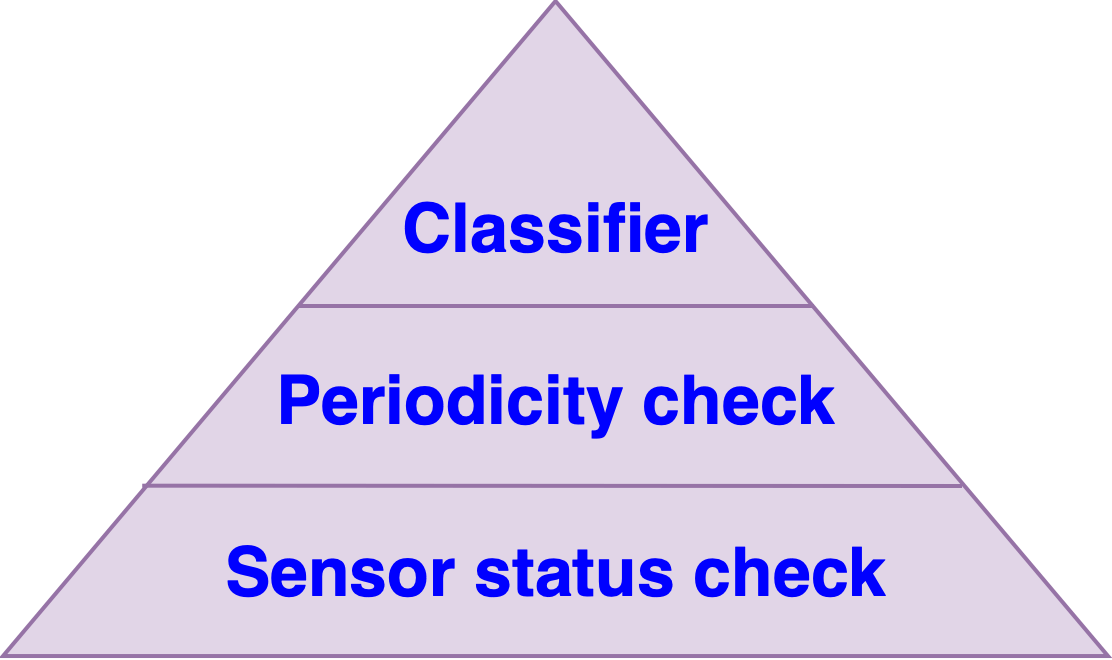
\includegraphics[width=0.4 \textwidth]{diagnostics_pyramid.png}
  \caption{Hierarchie subsystémů diagnostiky a detekce anomálií}
  \label{fig:diagnostics_pyramid}
\end{figure}  

Jednotlivé části diagnostického systému jsou popsány v této kapitole. Na \cref{fig:diagnostics} je zobrazena kompletní struktura všech úrovní diagnostického systému a jejich výstupy, které se zobrazují ve webové vizualizaci. Význam ikon (zelená, žlutá, červená) je popsán níže a webová stránka v \cref{chap:web_page}. 

\begin{figure}[H]
  \centering
  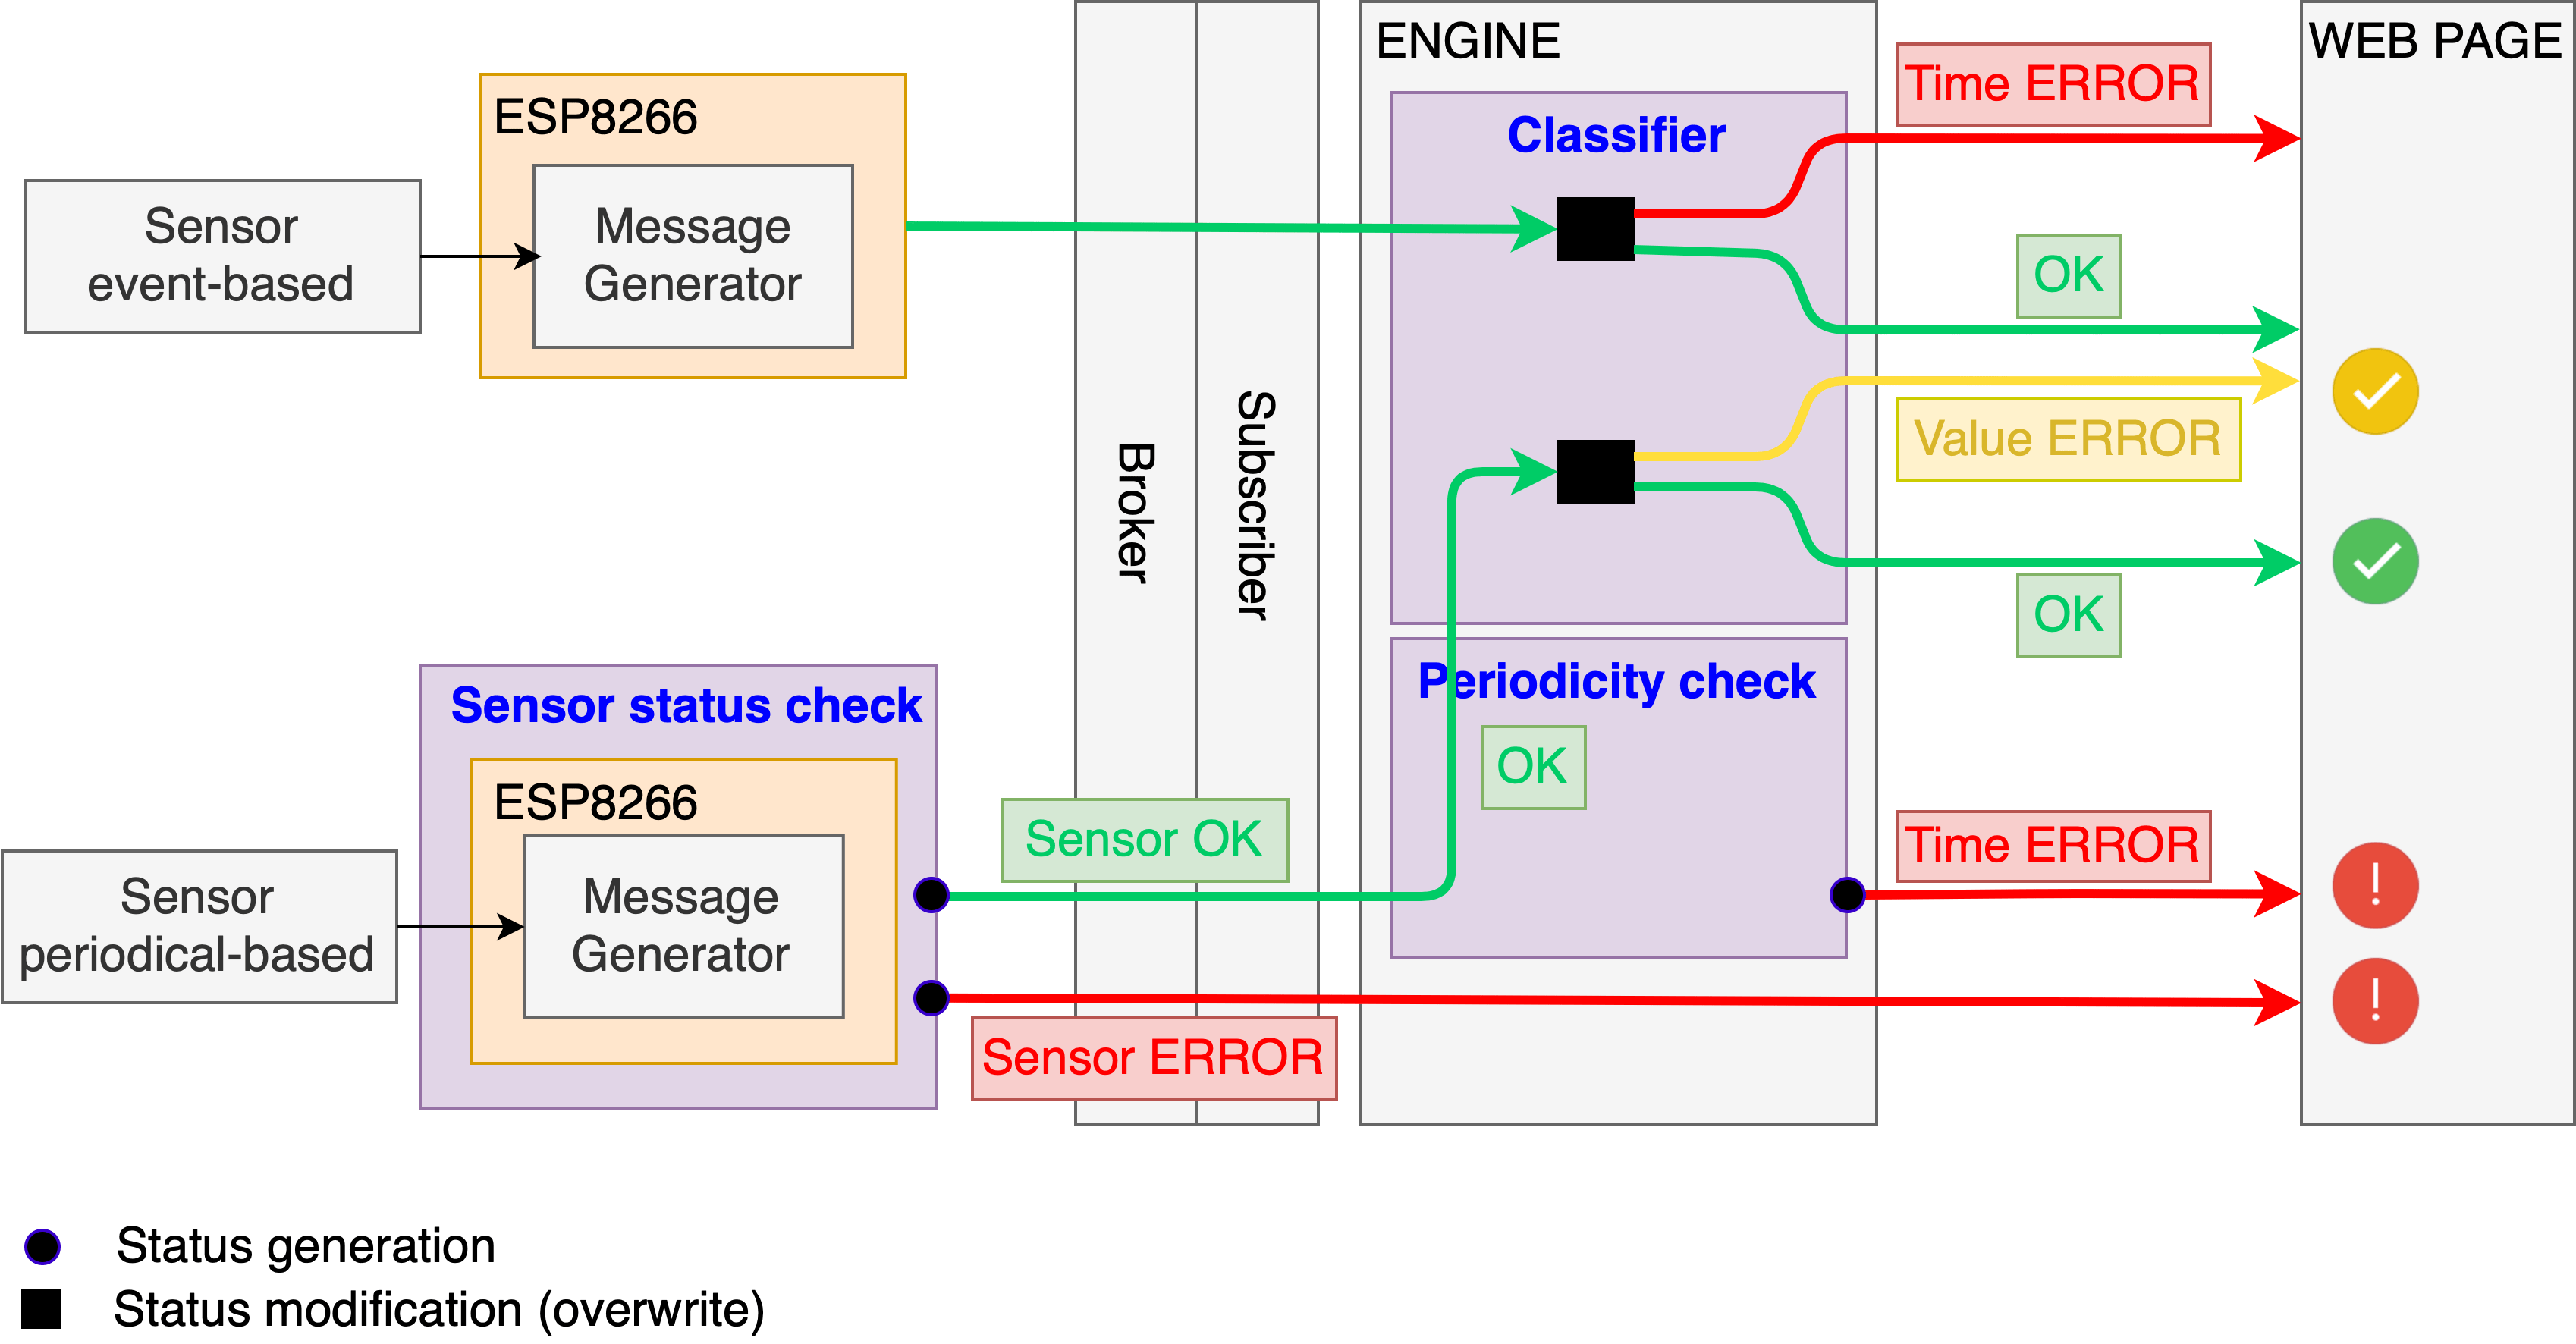
\includegraphics[width=1 \textwidth]{diagnostics.png}
  \caption{Struktura a popis všech úrovní diagnostického systému}
  \label{fig:diagnostics}
\end{figure}  

Diagnostický systém se skládá ze tří subsystémů. Detekce chyb na úrovni ESP8266 (\textit{Sensor status check}) je kontrola fyzického zapojení čidel s mikročipem a jejich funkčnost (detailní popis v \cref{sec:error_detection_esp}). Zbylé dvě úrovně diagnostického systému běží ve skriptu \textit{engine} na serveru. Subsystém kontroly periodicity zpráv na serveru (\textit{Periodicity check}) kontroluje, zda zprávy ze senzorů chodí pravidelně v očekávaných časových intervalech bez výpadků (popsáno v \cref{sec:periodicity_check}). Nad těmito dvěma subsystémy - detekce chyb na úrovni ESP8266 a kontrola periodicity příchozích zpráv je implementováno strojové učení ve formě klasifikace (\textit{Classifier}). Metody strojového učení na základě natrénovaných modelů klasifikují:

\begin{itemize}
	\item hodnoty (atribut \textit{value} v příchozí zprávě - \cref{subsec:message_structure}) u periodických zpráv (více v \cref{subsec:periodical_based_msg}).
	\item čas (atribut \textit{timestamp} v příchozí zprávě - \cref{subsec:message_structure}) u zpráv odesílaných na základě vzniku události (více v \cref{subsec:event_based_msg}). 
\end{itemize}

Tato nejvyšší úroveň diagnostiky - kontrola času a hodnot zpráv na základě strojového učení je popsána v \cref{sec:classifier}. 

\subsection*{Význam diagnostického systému}
Smyslem využití systému detekce anomálií je automatická diagnostika senzorů na základě příchozích zpráv. Výstupem tohoto systému jsou následující informace:

\begin{itemize}
 	\item Stav senzorů - zda je senzor online nebo offline. 
	\item Očekávaná periodicita - zda jsou zprávy ze senzorů odesílány pravidelně v očekávaných časech.
	\begin{itemize}
		\item U periodicky odesílaných zpráv podle zvolené periody.
		\item U zpráv odesílaných na základě vzniku události podle natrénovaného modelu.
	\end{itemize}
	\item Očekávaná hodnota - zda jsou hodnoty periodicky měřených veličin v očekávaném rozmezí podle natrénovaného modelu.
\end{itemize}

Tyto informace jsou na serveru dále zpracovávány a výsledné stavy (kombinace všech dostupných informací) jednotlivých senzorů se zobrazují ve formě ikon ve webové vizualizaci (více v \cref{chap:web_page}). \par
Uživatel dostává díky ikonám vedle měřených veličin okamžitý a kompletní přehled o stavu senzorů v chytré domácnosti a zároveň má jistotu, že data zobrazovaná na webové stránce jsou aktuální a relevantní, protože diagnostický systém ví, že data ze senzorů mají chodit pravidelně a když nové hodnoty nepřijdou, upozorní na to změnou ikony. Uživatel nemusí obnovovat webovou stránku a vždy se dozví, že senzor nepracuje stoprocentně a že zobrazená data nemusejí být relevantní. 

\subsection*{Výstup systému detekce anomálií} \label{subsec:diagnostics_output}
Výstupem systému diagnostiky chyb a detekce anomálií jsou stavy přiřazené jednotlivým senzorům. Stav senzoru může nabývat jedné z těchto tří hodnot.

\begin{itemize}
  \item [{
\includegraphics[align=c,scale=.18]{icon_ok}}] \textit{Sensor OK} je stav senzoru, kdy všechno funguje bezproblémově; Senzor odesílá data tak, jak se očekává - periodicky každou minutu a naměřená hodnota odpovídá natrénovanému modelu - zobrazeno na \cref{fig:diagnostics}; Ikona pro tento stav je zelená.
  \item [{
\includegraphics[align=c,scale=.18]{icon_value_error}}] Stav \textit{Value ERROR} nastává, pokud senzor odesílá data periodicky - tak, jak se očekává, ale naměřená hodnota je mimo předpovězený rozsah - neodpovídá natrénovaném modelu (žlutá šipka v \cref{fig:diagnostics}); Zobrazená hodnota veličiny je relevantní a aktuální, ale podle natrénovaného modelu jde o neočekávanou hodnotu. Neočekávaná hodnota znamená, že  hodnota naměřená tímto senzorem v tento denní čas je netypická - např. rozsvícení světla ve 3:00 ráno bude pravděpodobně klasifikováno jako neočekávané (mimo předpokládaný rozsah hodnot), pokud v minulosti ve 3:00 bylo vždy zhasnuto (strojové učení je popsáno v \cref{sec:classifier}); Ikona pro tento stav má žlutou barvu.
  \item [{
\includegraphics[align=c, scale=.18]{icon_error}}] \textit{Sensor ERROR} je status čidla, který nastává v momentě, kdy čidlo neposílá žádná data; Tento stav je způsobený buď výpadkem čidla (fyzické zapojení nebo porucha - \cref{sec:error_detection_esp}) nebo nepředpovídatelnými okolnostmi, které zamezují senzoru odesílat data (nedostupnost internetu, výpadek elektřiny); Tento status senzoru znázorňuje červená ikona.
\end{itemize}

Na \cref{fig:markovov_diagram} je zobrazeno schéma Markovova řetězce, který popisuje přechody mezi jednotlivými stavy senzorů. Z tohoto řetězce je patrné, že každý stav může přejít do libovolného jiného stavu nebo zůstat v aktuálním stavu. To znamená, že pokud se čidlo nachází v jednom momentě například ve stavu "sensor OK", v následujícím momentě se může nacházet opět ve stavu "OK"\ nebo v libovolném jiném stavu - "value ERROR"\ nebo "sensor ERROR".

\begin{figure}[H]
  \centering
  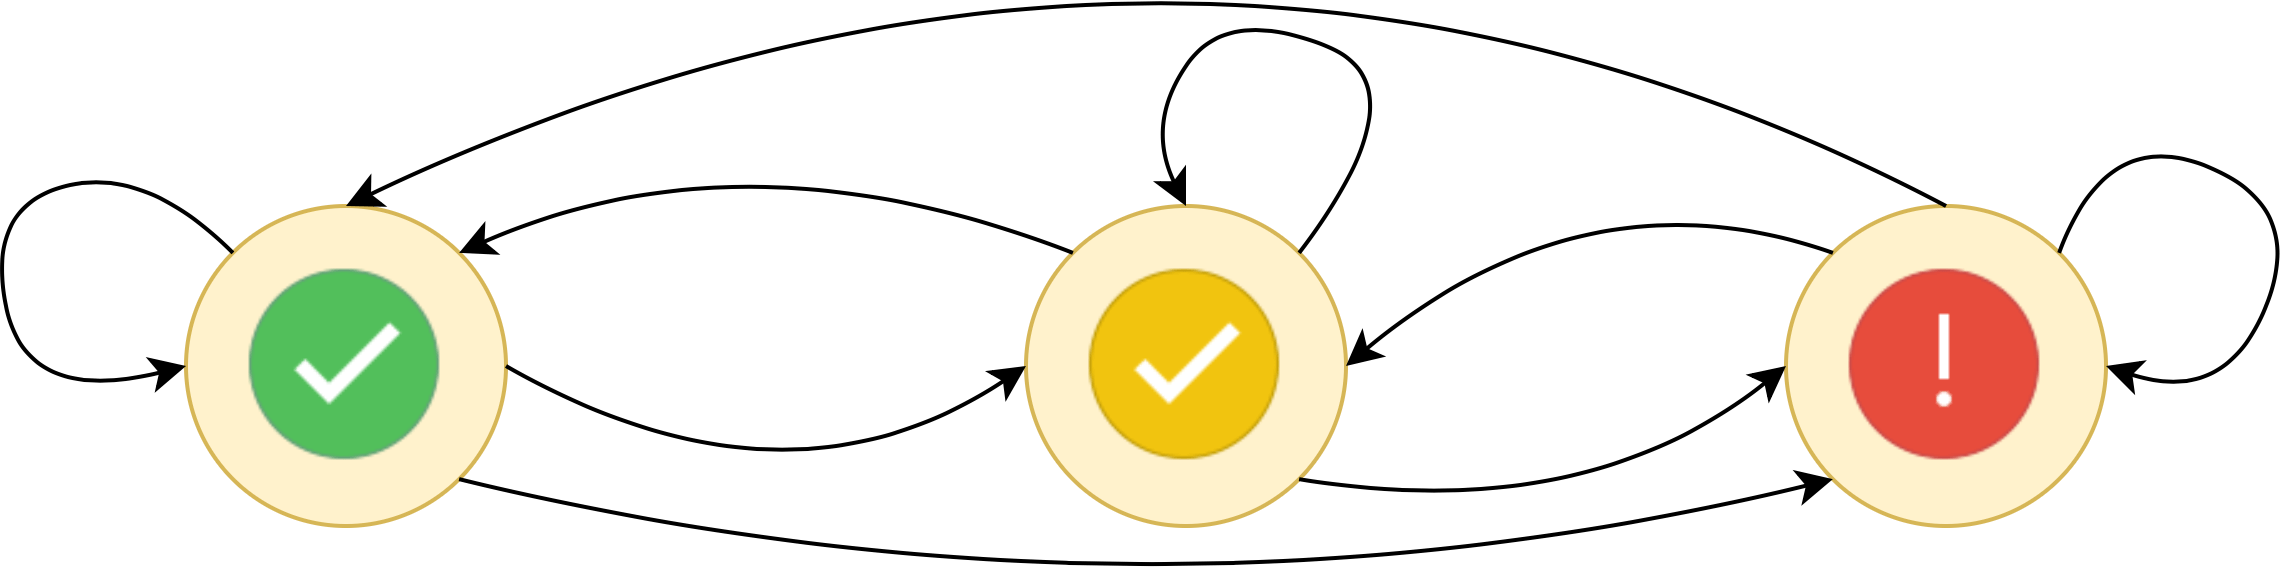
\includegraphics[width=0.6 \textwidth]{markovov_diagram.png}
  \caption{Markovův řetězec popisující přechody mezi jednotlivými stavy senzorů}
  \label{fig:markovov_diagram}
\end{figure}  

\section{Detekce chyb na úrovni ESP8266} \label{sec:error_detection_esp}
První a nejnižší úroveň diagnostiky jednotlivých senzorů je detekce chyb na úrovni samotného mikročipu. Tento systém je implementován na senzorech, které odesílají data periodicky (více v \cref{subsec:periodical_based_msg}). Mikročip ESP8266 při každém načítání dat z čidla zkouší, jestli z daného čidla lze načíst data a pozná, když je čidlo nefunkční. Čidlo se považuje za nefunkční, pokud při vyžádání naměřených dat nevrací žádné hodnoty. Tento stav čidla může být způsobený špatným zapojením, vypojením čidla nebo rozbitým čidlem. Implementace detekce chyb na úrovni mikročipu spočívá v obsluze výjimek v kódu. Část kódu, která řeší komunikaci s čidlem je obalena v \textit{try-except} bloku - mikročip se snaží načíst data z čidla a v případě, že to nelze, spadne kód do části \textit{except}, kde se obslouží výjimka tím, že se do proměnné, kam se ukládá naměřená hodnota, přiřadí číslo -1 (tento proces probíhá v části \textit{Get sensor status}, která je popsána na \cref{fig:esp_periodical_diagram}). Cyklus v kódu pokračuje dále k vytváření struktury zprávy, kde se testuje, zda se hodnota v proměnné nerovná -1. Pokud ano, ve zprávě se změní hodnota atributu "status"\ na "error"\ a senzor odešle zprávu. Senzor tedy odesílá zprávy na broker vždy - s funkčním i nefunkčním čidlem a status zprávy v detekci chyb na této úrovni nabývá pouze dvou hodnot - "ok"\ a "error". Výstup toho subsystému a náhled výsledných zpráv je zobrazen na \cref{fig:diagnostics_sensor_check}. Výstup z tohoto subsystému diagnostiky je dále zpracováván v metodě \textit{Periodicity check} nebo zobrazen na webové stránce - viz diagram na \cref{fig:diagnostics}.

\begin{figure}[H]
  \centering
  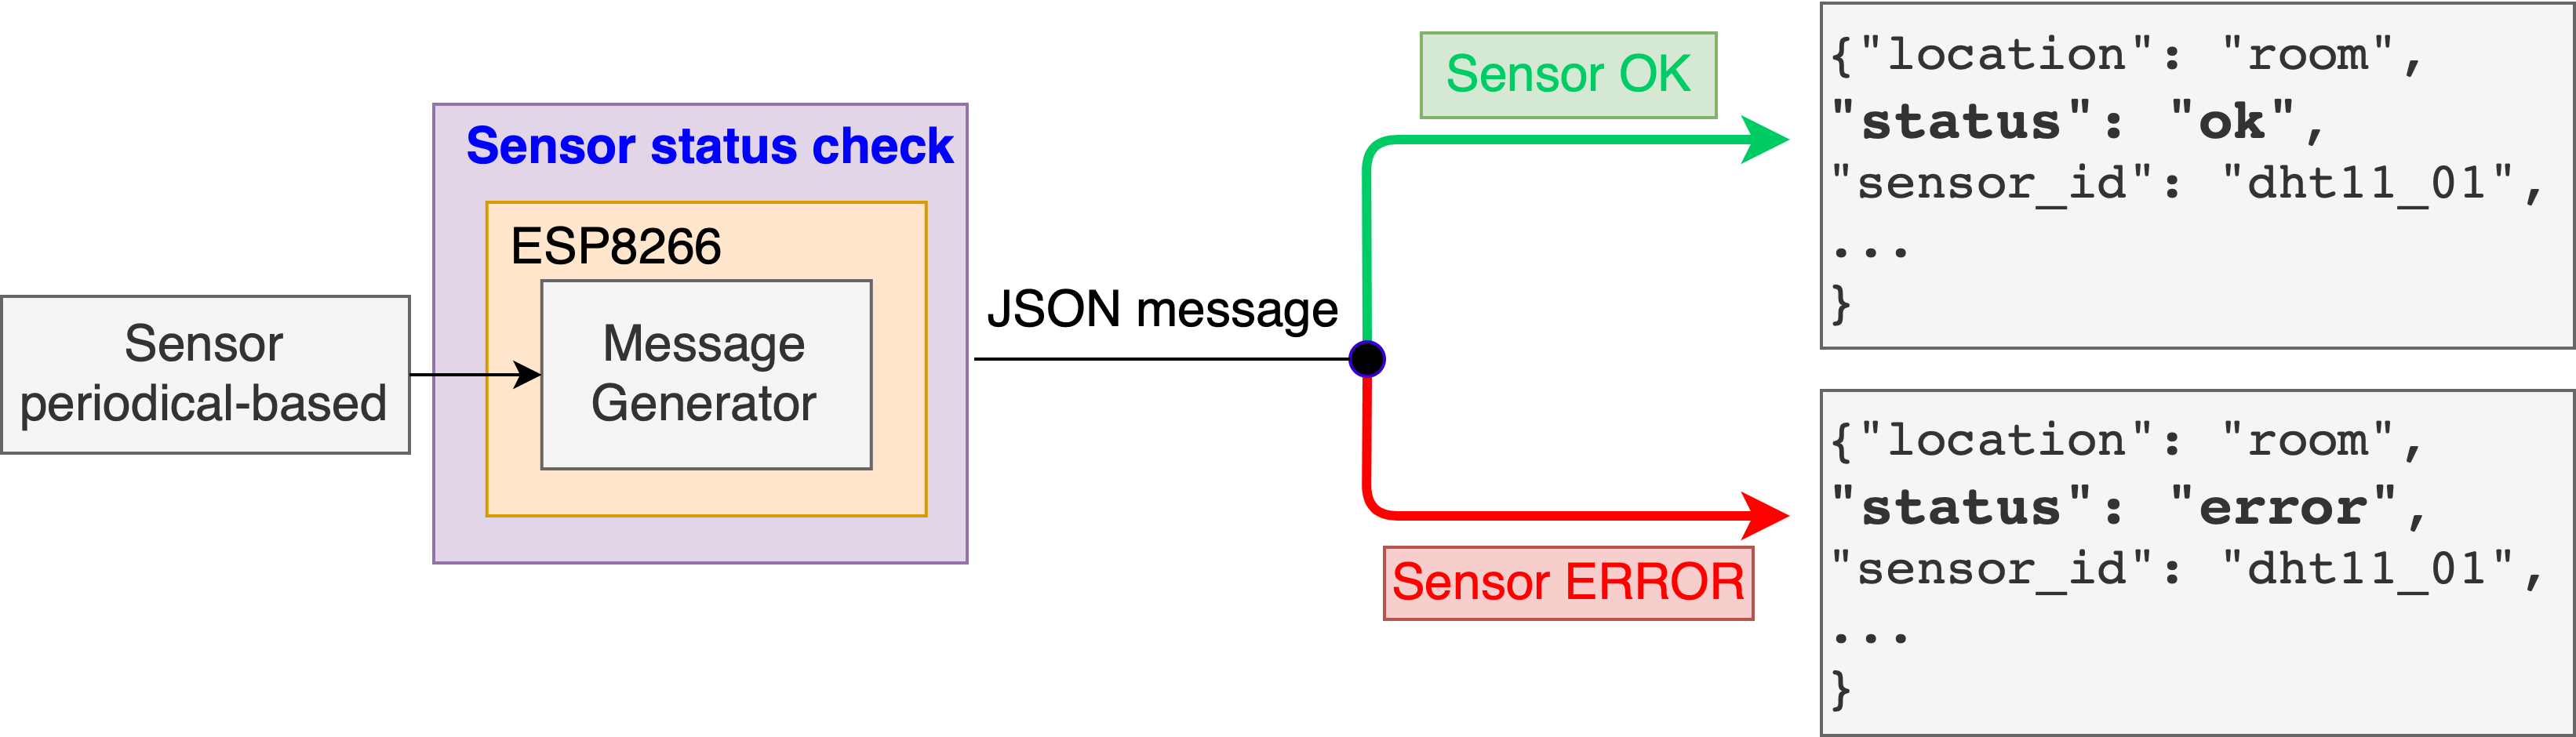
\includegraphics[width=1 \textwidth]{diagnostics_sensor_check.png}
  \caption{Výstupy subsystému detekce chyb na úrovni mikročipu ESP8266}
  \label{fig:diagnostics_sensor_check}
\end{figure} 

Implementací detekce chyb na úrovni mikročipu byla zajištěna robustnost senzorů. Jednotlivé senzory jsou odolné vůči výpadkům čidel - kód na mikročipu nespadne kvůli nefunkčnímu čidlu, jen se změní status zprávy. Díky tomu je také zajištěn nonstop provoz - čidla lze k ESP8266 připojovat a odpojovat (například čidlo teploty nebo magnetické kontakty, které jsou připojeny přes konektor) v reálném čase bez nutnosti restartu mikročipu. Pokud bude čidlo v jakémkoliv časovém okamžiku odpojeno a po chvíli zase připojeno, mikročip si s tím poradí. Změní se status zprávy a celý systém funguje dál. \par
Výhoda implementace detekce chyb na úrovni mikročipu se během testování ukázala několikrát. Například když bylo potřeba vyměnit nefunkční čidlo vlhkosti DHT11, které je připojené přes dutinkovou lištu (více v \cref{subsec:dht11}), jen se vyměnil kus za kus a senzor okamžitě začal načítat data z čidla a posílat naměřené hodnoty.

\section{Kontrola periodicity příchozích zpráv na \mbox{serveru}} \label{sec:periodicity_check}
Kontrola periodicity příchozích zpráv na serveru spočívá v implementaci funkce \textit{periodicity\_check}, která běží na serveru ve skriptu \textit{engine.py} (popsáno v \cref{sec:webserver}). Tento subsystém diagnostiky kontroluje pravidelnost odesílání dat ze senzoru na broker a současně pracuje s informací z diagnostického subsystému na úrovni mikročipu (popsáno v \cref{sec:error_detection_esp}) - viz diagram na \cref{fig:diagnostics}. Funkce \textit{Periodicity check} má k dispozici status zprávy - "sensor ok"\ nebo "sensor error". Jelikož u zpráv, které nenesou relevantní naměřené hodnoty (zprávy se statusem "sensor error") nemá smysl testovat jejich periodicitu, kontroluje se pravidelnost příchozích zpráv jen u zpráv se statusem "sensor ok". Kontrolu periodicity příchozích zpráv lze realizovat jen u periodicky odesílaných zpráv (popsáno v \cref{subsec:periodical_based_msg}), u zpráv odesílaných na základě vzniku události tato funkce z principu nemůže být využita. \par 
Pokud čidlo z neznámého důvodu neodešle zprávu nebo pokud se zpráva nepřenese k brokeru, informace o anomálii se přenese do webového rozhraní. Na \cref{fig:status_error} je ukázka příkladu zobrazení chyby senzoru ve webové vizualizaci. V případě chyby senzoru se změní ikona statusu a hodnota měřené veličiny je automaticky 0. Více o webové vizualizaci v \cref{sec:overview}.

\begin{figure}[H]
  \centering
  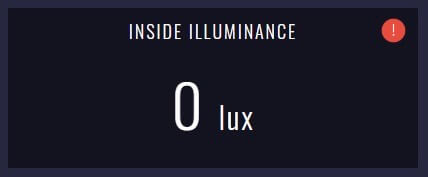
\includegraphics[width=0.4 \textwidth]{status_error.jpeg}
  \caption{Zobrazení ve webové vizualizaci v případě chyby senzoru}
  \label{fig:status_error}
\end{figure} 

Funkce \textit{periodicity\_check} čte všechny příchozí zprávy a porovnává čas poslední přijaté zprávy od daného čidla s aktuálním časem. Rozhodnutí o stavu čidla je prováděno podle následující formule: 

\[
    f(x)= 
\begin{cases}
    {
\includegraphics[align=c, scale=.15]{icon_ok}} \ \text{sensor ok}, & \text{if }  \triangle t \leq T [s]\\
    {
\includegraphics[align=c, scale=.15]{icon_error}} \ \text{sensor error}, & \text{if }  \triangle t > T [s],  \\
\end{cases}
\]

kde \( \triangle t = |t_1 - t_2| \) a $T$ je časová mez. Proměnná $t_1$ je čas poslední přijaté zpráv a $t_2$ je aktuální čas. Jestliže je rozdíl těchto dvou proměnných větší než zvolená mez, funkce detekuje chybu, do terminálu vypíše ID senzoru, ve kterém se vyskytuje chyba a status tohoto senzoru změní na "sensor ERROR". V opačném případě je senzor ve stavu "status OK". Na \cref{fig:diagnostics_periodical_check} lze vidět, že pokud je výstupem subsystému \textit{Periodicity check} hodnota stavu "sensor OK", je měřená veličina dále klasifikována metodami strojového učení (\textit{Classifier}) a pokud je výstupem "sensor ERROR", status se propíše na webovou stránku.

\begin{figure}[H]
  \centering
  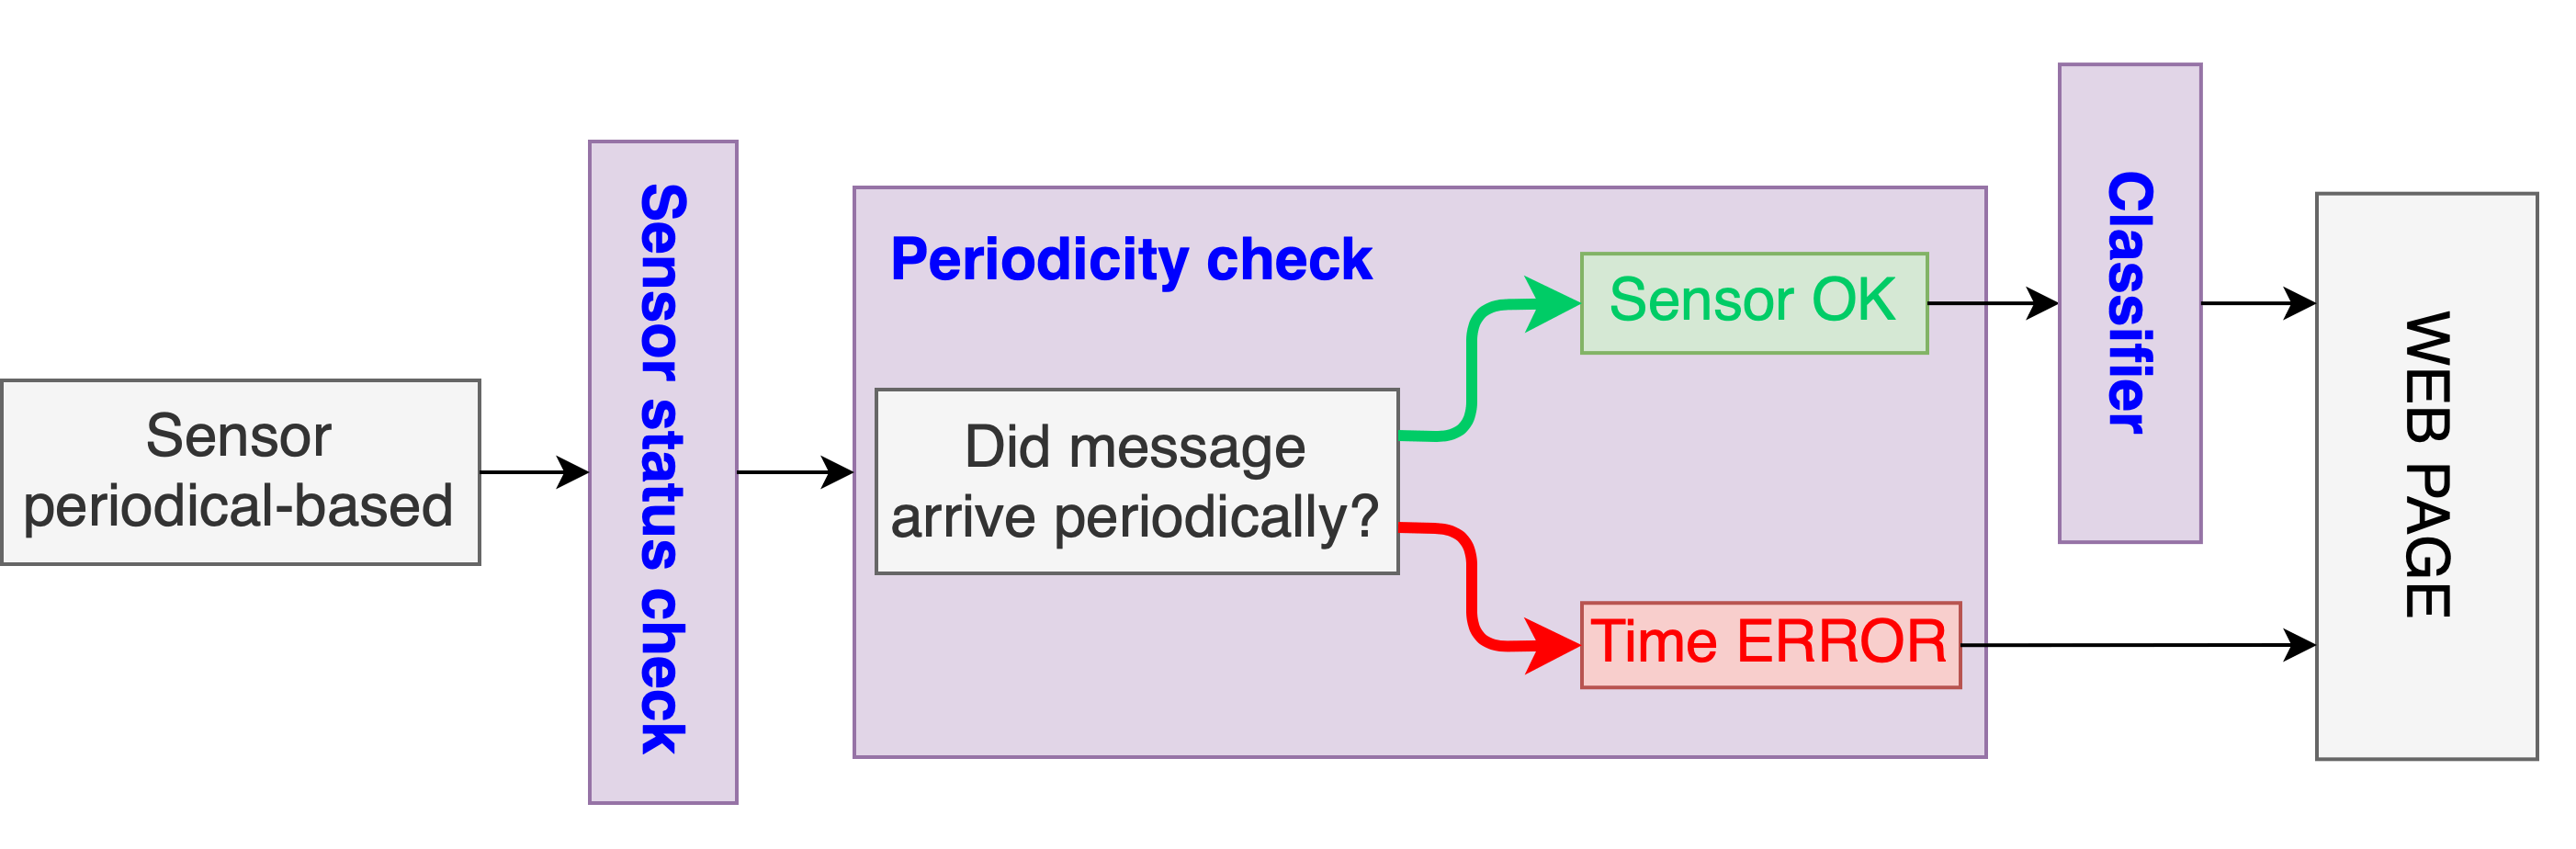
\includegraphics[width=0.9 \textwidth]{diagnostics_periodical_check.png}
  \caption{Výstupy subsystému kontroly periodicity příchozích zpráv}
  \label{fig:diagnostics_periodical_check}
\end{figure} 

V tomto projektu byla zvolena 60 vteřinová mez, což znamená, že stačí, aby senzor jednou neodeslal zprávu a na webové stránce se ikona statusu toho senzoru hned změní na červenou. Toto kritérium je relativně přísné, v běžném provozu by stačilo mez volit například 180 vteřinovou, tudíž by se ve webovém rozhraní zobrazoval senzor jako aktivní i když by dvakrát neodeslal zprávu. Tři minuty stará data lze považovat za stále aktuální a stav senzorů by byl více konzistentní - občas se stane (ne příliš často, například jednou za 2 dny provozu), že senzor z nějakého důvodu nestihne odeslat zprávu v dané minutě a webová vizualizace ho ihned vyhodnotí jako nefunkční, přitom senzor v dalších minutách opět zprávy odesílá. Dochází k rychlé změně statusu senzoru a uživatel by mohl být zmatený. Volba hodnoty časové meze je kompromisem mezi uživatelskou přívětivostí a naprosto přesnou indikací stavu. 

\section{Kontrola času a hodnot zpráv na základě \newline strojového učení} \label{sec:classifier}
Detekce anomálií na základě klasifikace spočívá v implementaci metod strojového učení. Příchozí zprávy jsou pomocí natrénovaného modelu klasifikovány a informace o klasifikaci je přidána do struktury zprávy (struktura zprávy je popsána v \cref{subsec:message_structure}) - do zprávy je přidán atribut \textit{classification}, který nabývá hodnot 1 a -1. \par
Metody strojového učení jsou v diagnostickém systému implementovány pro kontrolu:

\begin{itemize}
	\item času u měřených veličin, které jsou odesílány na základě vzniku události (např. pohyb v místnosti) - \textit{1D veličiny}
	\item hodnot u měřených veličin, které jsou odesílány pravidelně s pevnou periodou (např. vnitřní teplota) - \textit{2D veličiny}
\end{itemize}

Kontrola času měřených veličin probíhá na základě natrénovaného modelu a kontrola hodnoty na základě očekávaných hodnot získaných z natrénovaného modelu. Veličiny, které jsou měřeny v rámci projektu chytré domácnosti můžeme rozdělit do dvou kategorií - jednodimenzionální a dvoudimenzionální.

\subsection{1D veličiny} \label{subsec:1D_quantities}
1D data jsou veličiny, které jsou odesílány na server na základě vzniku události. Mezi tyto veličiny patří v tomto projektu detekce pohybu v místnosti, status okna (otevřené nebo zavřené) a status dveří (otevřené nebo zavřené). Přestože tyto události nevznikají periodicky s předem stanovenou periodou, je u nich kontrolován čas odeslání zprávy. Kontrola času, kdy nastane událost má u těchto veličin smysl, protože ačkoliv vznik těchto událostí není čistě periodický, jistá pravidelnost se zde objevuje. Při pozorování chování členů domácnosti lze odvodit opakující se vzorce. Například pohyb v místnosti je detekován v určité části dne mnohem častěji než v jinou chvíli (během dopoledne všedních pracovní dnů je pohyb v domácnosti detekován zpravidla výjimečně, protože členové domácnosti jsou v zaměstnání nebo ve škole). Stejný princip je u otevírání okna a dveří. V určitých časech během dne je intenzita otevírání oken a dveří větší a mnohem pravděpodobnější, než v jinou chvíli. Po sesbírání nutného minimálního počtu vzorků dat je na základě těchto jevů natrénován model, který je následně využitý k predikování času vzniku události. Časové období, ve kterém budou sbírána data a následně trénován model, může být například jeden měsíc a pokud člen domácnosti po dobu tohoto měsíce bude otevírat okno pravidelně například jednou denně večer a po zbytek dne bude okno zavřené, natrénovaný model bude následující zprávy klasifikovat na základě tohoto chování - pokud bude okno otevřené ve stejnou chvíli jako doposud, zpráva bude klasifikována jako důvěryhodná. Pokud bude okno otevřené například v průběhu noci (během trénovaní modelu tato situace nikdy nenastala), bude zpráva klasifikována jako nedůvěryhodná.\par
Čas vzniku události je na základě natrénovaného modelu porovnáván s očekávaným časem, tzn. veličiny, jejichž hodnoty se mění na základě vzniku události, jsou zaznamenány v nějakém čase a jsou klasifikovány podle toho, zda čas odpovídá natrénovanému modelu (zda model předpokládá, že vznik události v tomto čase je statisticky pravděpodobný). \par
Pokud je zpráva klasifikována jako důvěryhodná, atribut \textit{classification} ve zprávě obsahuje hodnotu 1. V opačném případě, kdy je zpráva klasifikována jako nedůvěryhodná, je atributu přiřazena hodnota 1. Výstupy toho subsystému jsou zobrazeny na \cref{fig:diagnostics_1D}.

\begin{figure}[H]
  \centering
  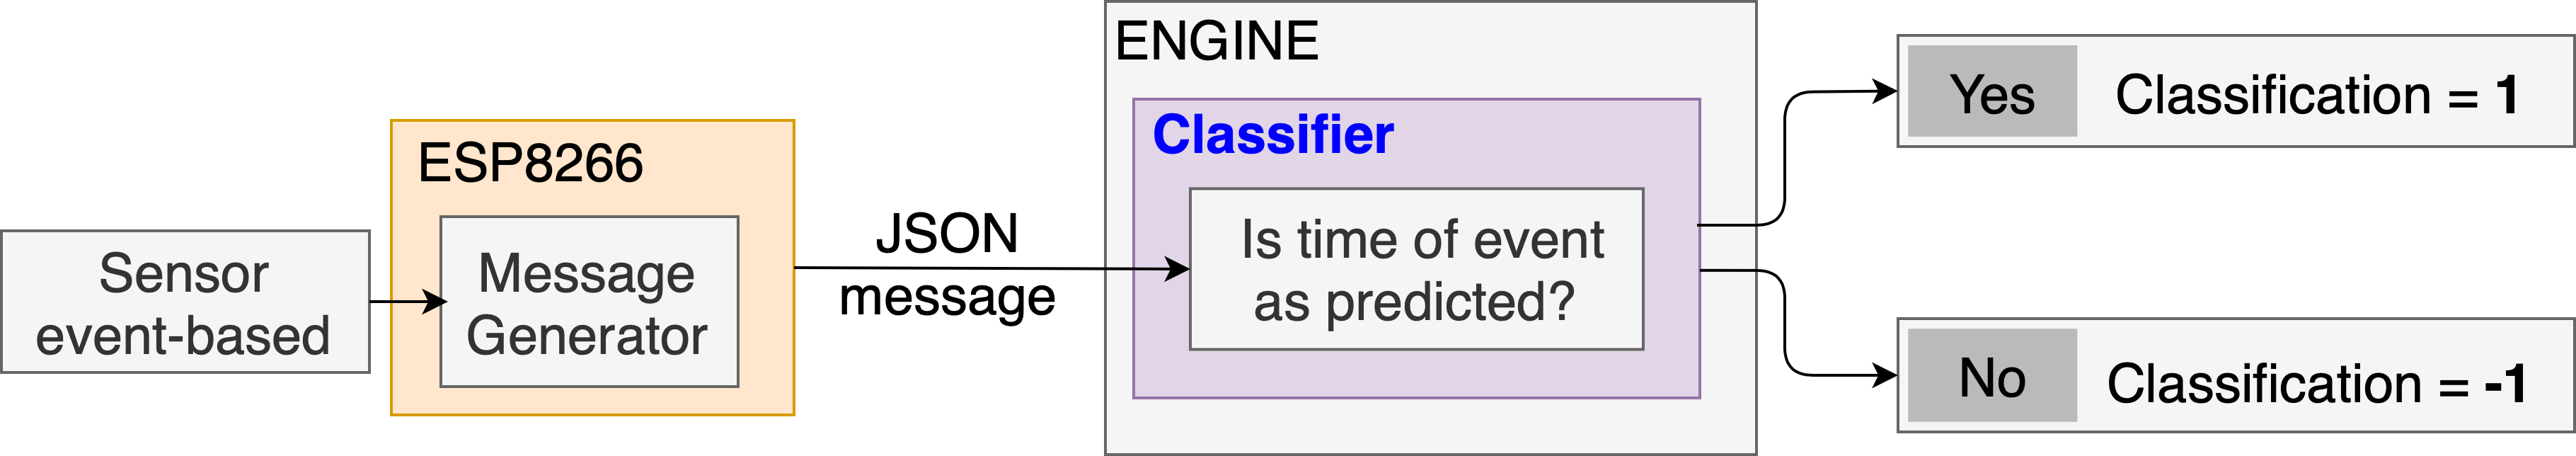
\includegraphics[width=1 \textwidth]{diagnostics_1D.png}
  \caption{Výstupy subsystému klasifikace z natrénovaného modelu u 1D veličin}
  \label{fig:diagnostics_1D}
\end{figure}  

Z diagramu na \cref{fig:diagnostics} je vidět, že zprávy z těchto senzorů jsou zpracovávány pouze subsystémem \textit{Classifier} a výstupem systému diagnostiky stavu těchto senzorů je hodnota klasifikace 1 nebo -1 podle důvěryhodnosti času vzniku události. 

Na \cref{fig:1D_window_open} je zobrazen graf sledující veličinu \textit{status okna}. Status okna nabývá dvou hodnot - otevřené nebo zavřené a následující graf ilustruje očekávané (predikované) denní hodnoty této veličiny na základě klasifikace z natrénovaného modelu. Na vodorovné ose jsou naneseny časové hodnoty v hodinách (0 až 24) a na svislé ose je zobrazena pravděpodobnost (0 až 0,2). 

\begin{figure}[H]
  \centering
  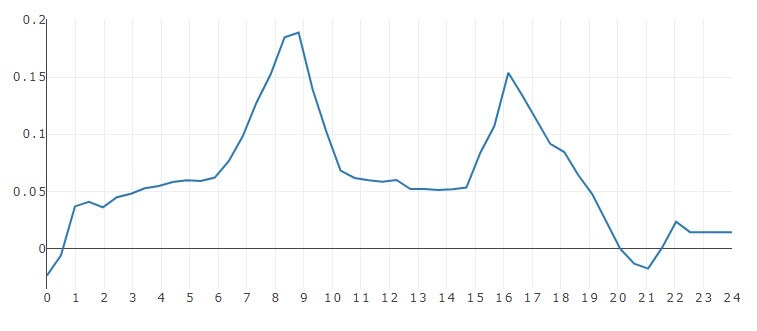
\includegraphics[width=1 \textwidth]{1D_window_open.jpeg}
  \caption{Graf ilustrující očekávané denní hodnoty podle natrénovaného modelu pro veličinu \textit{status okna}}
  \label{fig:1D_window_open}
\end{figure}  

Tento graf ukazuje s jakou pravděpodobností natrénovaný model očekává změnu statusu okna v závislosti na části dne. Čím výše se křivka pohybuje, tím více je pravděpodobné, že dojde ke změně statusu okna. Například v čase od 7 do 9 hodin ráno je velmi pravděpodobné, že dojde ke změně statusu (ráno pravděpodobně uživatel otevře okno). Podobně je tomu v úseku od 16 do 18 hodin. Naopak v době od 20 do 21 hodin model neočekává změnu statusu (obyvatel domácnosti v tuto denní dobu nejspíš neotevírá nebo nezavírá okno) - pravděpodobnost je menší než 0. \par
Na stejném principu funguje klasifikace veličin \textit{status dveří} a \textit{pohyb v místnosti}. Na základě predikovaných hodnot z natrénovaného modelu lze s určitou pravděpodobností předpovídat, kdy je v místnosti často pohyb osob nebo kdy je pravděpodobné, že uživatel zavře dveře. \par
U 1D veličin klasifikace slouží ke kontrole \underline{času} vzniku události.

\subsection{2D veličiny} \label{subsec:2D_quantities}
2D data jsou veličiny, které jsou odesílány periodicky. V projektu chytré domácnosti je to například měřená teplota, jejíž měření a odesílání hodnot se opakuje pravidelně každou minutu (více o těchto veličinách v \cref{subsec:periodical_based_msg}). U 2D periodických veličin slouží klasifikace ke kontrole hodnot přicházejících zpráv, které jsou porovnávány s očekávanými hodnotami na základě natrénovaných modelů. Kontrola času (periodicity) u těchto veličin je prováděna externě v subsystému \textit{Periodicity check} (více v \cref{sec:periodicity_check}). \par
Jelikož zprávy z těchto čidel jsou odesílány často, lze po krátké době sesbírat dostatečné množství dat, ze kterého je možné následně natrénovat modely. Hodnoty těchto veličin se odvíjejí od domácího prostředí a lze je poměrně přesně predikovat - například teplota v místnosti je udržována v úzkém rozmezí několika stupňů a v průběhu dne se mění velmi málo. Na základě sesbíraných dat, ze kterých je natrénován model pro danou veličinu, jsou klasifikovány všechny další příchozí zprávy. Například model pro kontrolu relevantnosti hodnot vnitřní teploty je natrénován z dat, kdy typická vnitřní teplota může být v rozmezí 23 až 25 \si{\degree}C. Pokud další zpráva, která přijde z tohoto čidla bude mít informaci o hodnotě teploty v místnosti 24 \si{\degree}C, je klasifikována jako věrohodná, atributu \textit{classification} je přiřazena hodnota 1 a ve webové vizualizace se zobrazí zelená ikona. Když následně přijde další zpráva, která nese informaci o hodnotě vnitřní teploty 30  \si{\degree}C, bude klasifikována jako nedůvěryhodná, protože natrénovaný model tuto hodnotu statisticky nepředpokládá. Atributu \textit{classification} bude přiřazena hodnota -1 a na webové stránce se zobrazí žlutá ikona - uživatel je informován, že senzor odeslal zprávu, ale hodnota měřené veličiny je mimo předpovězený rozsah a tudíž nepravděpodobná. \par
Na \cref{fig:diagnostics_2D} jsou zobrazeny jednotlivé subsystémy, přes které projde zpráva odeslána senzorem, který posílá zprávy pravidelně. Ze schématu lze vidět, že odeslaná zpráva projde přes všechny tři subsystémy - \textit{Sensor status check}, \textit{Periodicity check} a \textit{Classifier}. Výstupem subsystému kontroly hodnot zpráv pro 2D veličiny (\textit{Classifier}) je hodnota atributu \textit{classification} -1 nebo 1. Tato informace je následně dále zpracovávána ve webovém rozhraní. 

\begin{figure}[H]
  \centering
  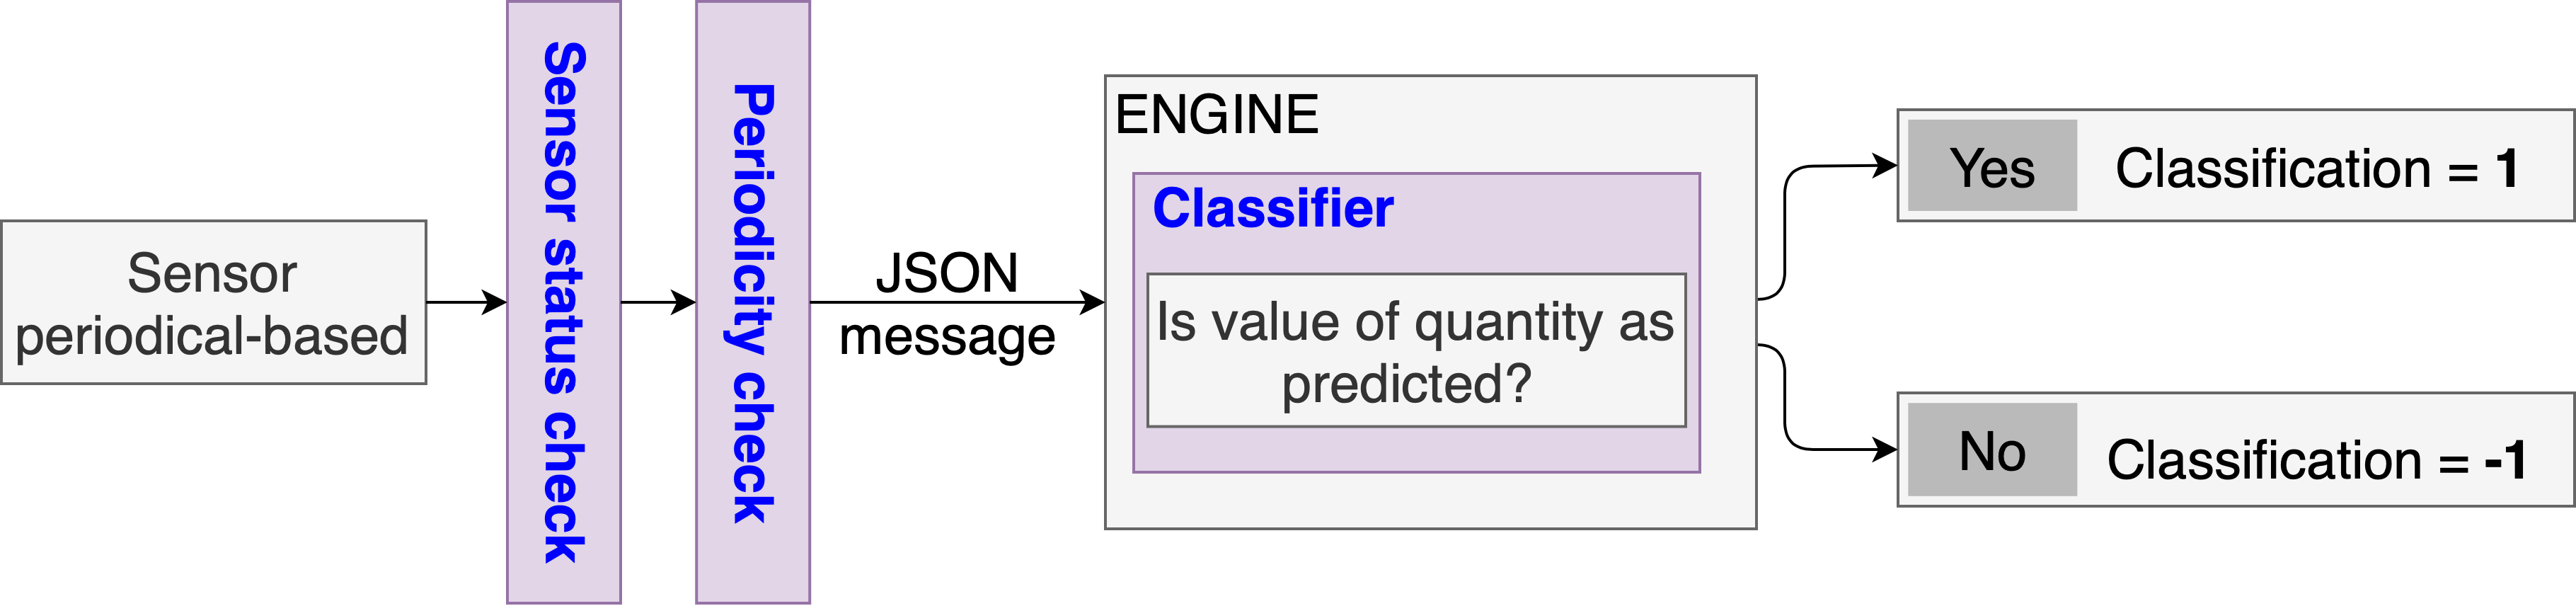
\includegraphics[width=1 \textwidth]{diagnostics_2D.png}
  \caption{Výstupy subsystému klasifikace z natrénovaného modelu u 2D veličin}
  \label{fig:diagnostics_2D}
\end{figure}  

Pokud se tedy na webové stránce u 2D veličin (například teplota v místnosti) zobrazuje zelená ikona, lze s jistotou říci, že zobrazovaná hodnota je aktuální a důvěryhodná, protože tato hodnota prošla třemi vrstvami diagnostického subsystému a ve všech subsystémech byla vyhodnocena kladně. \par
Klasifikace naměřených hodnot jako nevěrohodných může vzniknout z více důvodů. Buď je čidlo vadné a posílá hodnoty měřené veličiny, které nekorespondují s realitou nebo je trénovaný model zastaralý (například při změně ročního období a použití staršího modelu) a nebo jde o anomálii, která nebyla předvídatelná. Nepředvídatelná anomálie (nepředvídatelné chování) se často vyskytuje například u senzoru vnitřního osvětlení. Model natrénovaný z dat ze senzoru intenzity vnitřního osvětlení je například natrénován na situaci, kdy člen domácnosti rozsvítí světlo pravidelně ve večerních hodinách a zhasíná okolo 22:00. Pokud obyvatel domu výjimečně rozsvítí v noci, tato zpráva bude klasifikována jako nevěrohodná s hodnotou \textit{classification} -1. V tomto případě nejde o chybu čidla, ale o nepředvídatelnou hodnotu, která vybočuje z mezí stanovených natrénovaným model (pokud ovšem člen domácnosti zapíná světlo pravidelně každou noc ve stejnou dobu, tato zpráva již bude klasifikována jako věrohodná). Na základě těchto dat lze kvalitně predikovat chování a události v chytré domácnosti. \par
Na \cref{fig:2D_temperature} je graf ilustrující očekávané (predikované) denní hodnoty podle natrénovaného modelu pro teplotu v místnosti. Na vodorovné ose jsou naneseny časové hodnoty v hodinách (0 až 24) a na svislé ose jsou hodnoty teploty (10 až 30) ve stupních Celsia. Ve vertikálním sloupci jsou barevně zobrazeny pravděpodobnosti, se kterými model očekává denní hodnoty vnitřní teploty. 

\begin{figure}[H]
  \centering
  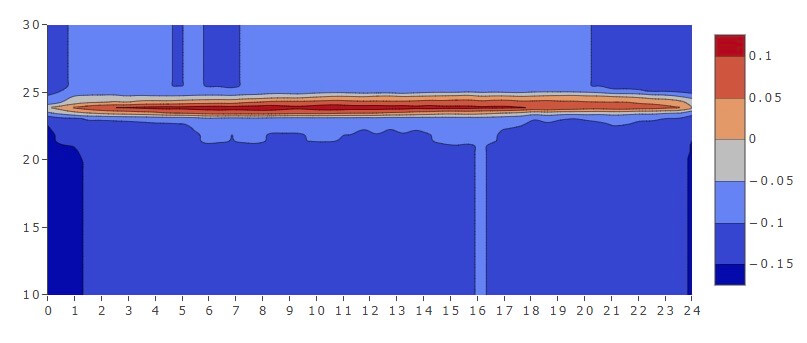
\includegraphics[width=1 \textwidth]{2D_temperature.jpeg}
  \caption{Graf ilustrující očekávané denní hodnoty podle natrénovaného modelu pro veličinu \textit{vnitřní teplota}}
  \label{fig:2D_temperature}
\end{figure}  

Z grafu lze vidět, že teplota uvnitř místnosti se pohybuje s největší pravděpodobností od přibližně 23 do 25 \si{\degree}C. V této oblasti jsou hodnoty zobrazeny červeně. Teplota 24 \si{\degree}C je statisticky nejvíce očekávaná s hodnotou pravděpodobnosti 0.1 - této hodnoty teplota v místnosti dosahovala při trénování modelu nejčastěji. Natrénovaný model tedy očekává denní hodnoty vnitřní teploty s vysokou pravděpodobností právě v tomto rozmezí od 23 do 25 \si{\degree}C. Ostatní plocha, která je zobrazena modře, znázorňuje, že v této oblasti jsou hodnoty vnitřní teploty velmi nepravděpodobné. Tento model klasifikuje nové příchozí hodnoty vnitřní teploty jako věrohodné (\textit{classification} 1), pokud se nacházejí v blízkém okolí rozmezí 23 až 25 \si{\degree}C a jako nedůvěryhodné (\textit{classification -1}), pokud se vyskytují jinde. \par
Na stejném principu funguje klasifikace veličin \textit{vnitřní a venkovní teplota}, \textit{vlhkost}, \textit{barometrický tlak} a \textit{intenzita osvětlení}. Na základě predikovaných hodnot z natrénovaného modelu lze s určitou pravděpodobností předpovídat, jakých hodnot budou měřené veličiny nabývat. \par
Výstupem tohoto subsystému je kromě informace o relevantnosti očekávaných hodnot několik zajímavých faktů. Z dlouhodobého hlediska bylo například vypozorováno, že vlhkost v místnosti se mění s ročním obdobím - v zimě je kolem 40 - 50 \%, v létě je v rozmezí okolo 20 - 30 \%. U vlhkosti je dále zajímavé, že pokud je místnost prázdná, hodnota vlhkosti je téměř konstantní a po vstupu člověka do místnosti vlhkost vzroste o jednotky procent. S touto informací by se teoreticky dalo pracovat dále například v rámci rozšíření prvků bezpečnosti (detekce osob nejen pomocí PIR čidla). \par
U 2D veličin klasifikace slouží ke kontrole \underline{hodnot} měřených veličin. 

\subsection*{Hierarchie statusů}
Ve webovém rozhraní se mění ikony statusu podle tří výše definovaných stavů (\textit{sensor ok}, \textit{value error}, \textit{sensor error}). Statusy se mohou navzájem přepisovat podle hierarchie důležitosti, která je následující.  \par

\begin{lstlisting}[language=json]
	   Sensor ERROR > Value ERROR > Sensor OK
\end{lstlisting}

To znamená, že pokud senzor například odešle zprávu se statusem "sensor OK", ale hodnota měřené veličiny je klasifikována jako -1, na webu se zobrazí status odpovídající klasifikaci -1 - "value ERROR", protože status "value ERROR"\ má větší váhu, než status "sensor OK". \par
Pokud senzor odešle zprávu se statusem "sensor ERROR", tato zpráva není dále klasifikována a na webové stránce se zobrazí ikona "sensor ERROR". Váha tohoto statusu je nejvyšší. \par
Pokud senzor odešle zprávu se statusem "sensor OK"\ a klasifikátor přiřadí hodnotu 1, ikona statusu na webu zůstává "sensor OK". \par
Když senzor odešle zprávu se statusem "sensor OK", ale pak několik minut po sobě přestane odesílat zprávy, na webu se status změní na "sensor ERROR". \par
Diagnostika a změny ikon zpráv jsou zkrátka řešeny tak, aby to bylo pro uživatele přirozené a na první pohled pochopitelné. Zelená ikona znamená, že je všechno v pořádku. Žlutá ikona indikuje, že je senzor funkční a odeslal naměřená data, akorát natrénovaný model tuto hodnotu naměřenou v tento denní čas vyhodnotil jako neočekávanou. Pro uživatele to znamená, že zobrazená data jsou relevantní a aktuální, ale podle klasifikátoru se vychylují od rozmezí hodnot, kterých tato veličina v této části dne obvykle nabývá. Červená ikona uživatele varuje a říká, že je senzor nefunkční. Diagnostický systém kombinuje vstupy ze systému detekce chyb čidel (\textit{Sensor status check}) s kontrolou  pravidelnosti odesílaných zpráv (\textit{Periodicity check}) a kontrolou věrohodnosti posílaných zpráv (\textit{Classifier}). Kombinací těchto tří subsystémů generuje výstupní ikony na webové stránce, které informují uživatele. Kromě informací generovaných z tohoto systému diagnosticky se ve webovém rozhraní zobrazují grafy predikce budoucího vývoje sledované veličiny. 

